\chapter{Discussion}
    \section{Robot displacement}
        The results of leg patterns from Section \ref{sec:res_legs} does correlate with the theoretical results expected when processing the potential energy \cite{mo_main_paper}. Also regarding specifically sequences A and B, the experimental robot could validate the correct implementation in the code. In particular, it was experimentally demonstrated that the forward and backward motion could be achieved when using the robot a specific configurations. Forward motion was achieved using the four joints in sequence A, and the backward motion was achieved using the four joints in sequence B. As shown on Figure \ref{fig:robot_position}, the simulation results gives very similar results to the experimental video, with a backward motion and almost no change in the y-axis or in the orientation of the robot. During the cycle the robot had some orientation changes that can also be seen on the videos.\\
        
        The friction model implemented using weight ratio as a coefficient of displacement for each touching leg seems to gives interesting results. Basics examples, such as forward motion, or no motion at all are produced as expected with the model. Especially it behaves correctly with two or four legs that are touching the floor. It would be interesting to see how well they correlate with the real world experiment, as some of the experiments were not possible to run at this time. Depending on the results and the correlation to future experiments, it asks for some adjustments. The robot displacement model should be good enough to provide information to the Deep Q Learning Controller as a pre-training process before using a second training process with a real robot.\\
        
        Simulation's performance is also sufficient. A cycle of simulation takes a few seconds on to generate (video included). The configuration files also allows to change the dimension of the robot at a specific place and also to modify the simulation scheme.
        
    \section{Motion Mapping}
        Results from Section \ref{sec:res_mapping} shows that the robot can move in x-axis, y-axis and change its orientation depending on the choice of sequences and actuation. Displacement in the x-axis are included between $-10cm$ and $+0.8cm$, while the displacement in the y-axis are lower ($-0.9cm$ to $+0.9cm$). This difference between the two axis can be explained by the difference of motion of each joint in the respective axis. The change of orientation of the robot goes from $-6$° to $+6$° per cycle, which should be enough to be observable in experiments. 
        
        It is interesting to see how the robot behaves when we only changes the phase difference of the actuators. As shown on Figure \ref{fig:displacement_spread}. If a phase difference is selected between the actuators (phase 180°), it limits the displacement of the robot along its x-axis. It does not restrict specifically the displacement along y-axis or the change in the orientation of the robot. A second interesting result that can be observed on Figure \ref{fig:displacement_spread} is the correlation between a y-axis displacement and the orientation (yaw) of the robot. This Figure shows that if there is no phase difference, there is a positive correlation between those two output. If the phase difference is equal to 180°, there is an inverted correlation between those axis. \\
        
        \begin{figure}
            \centering
            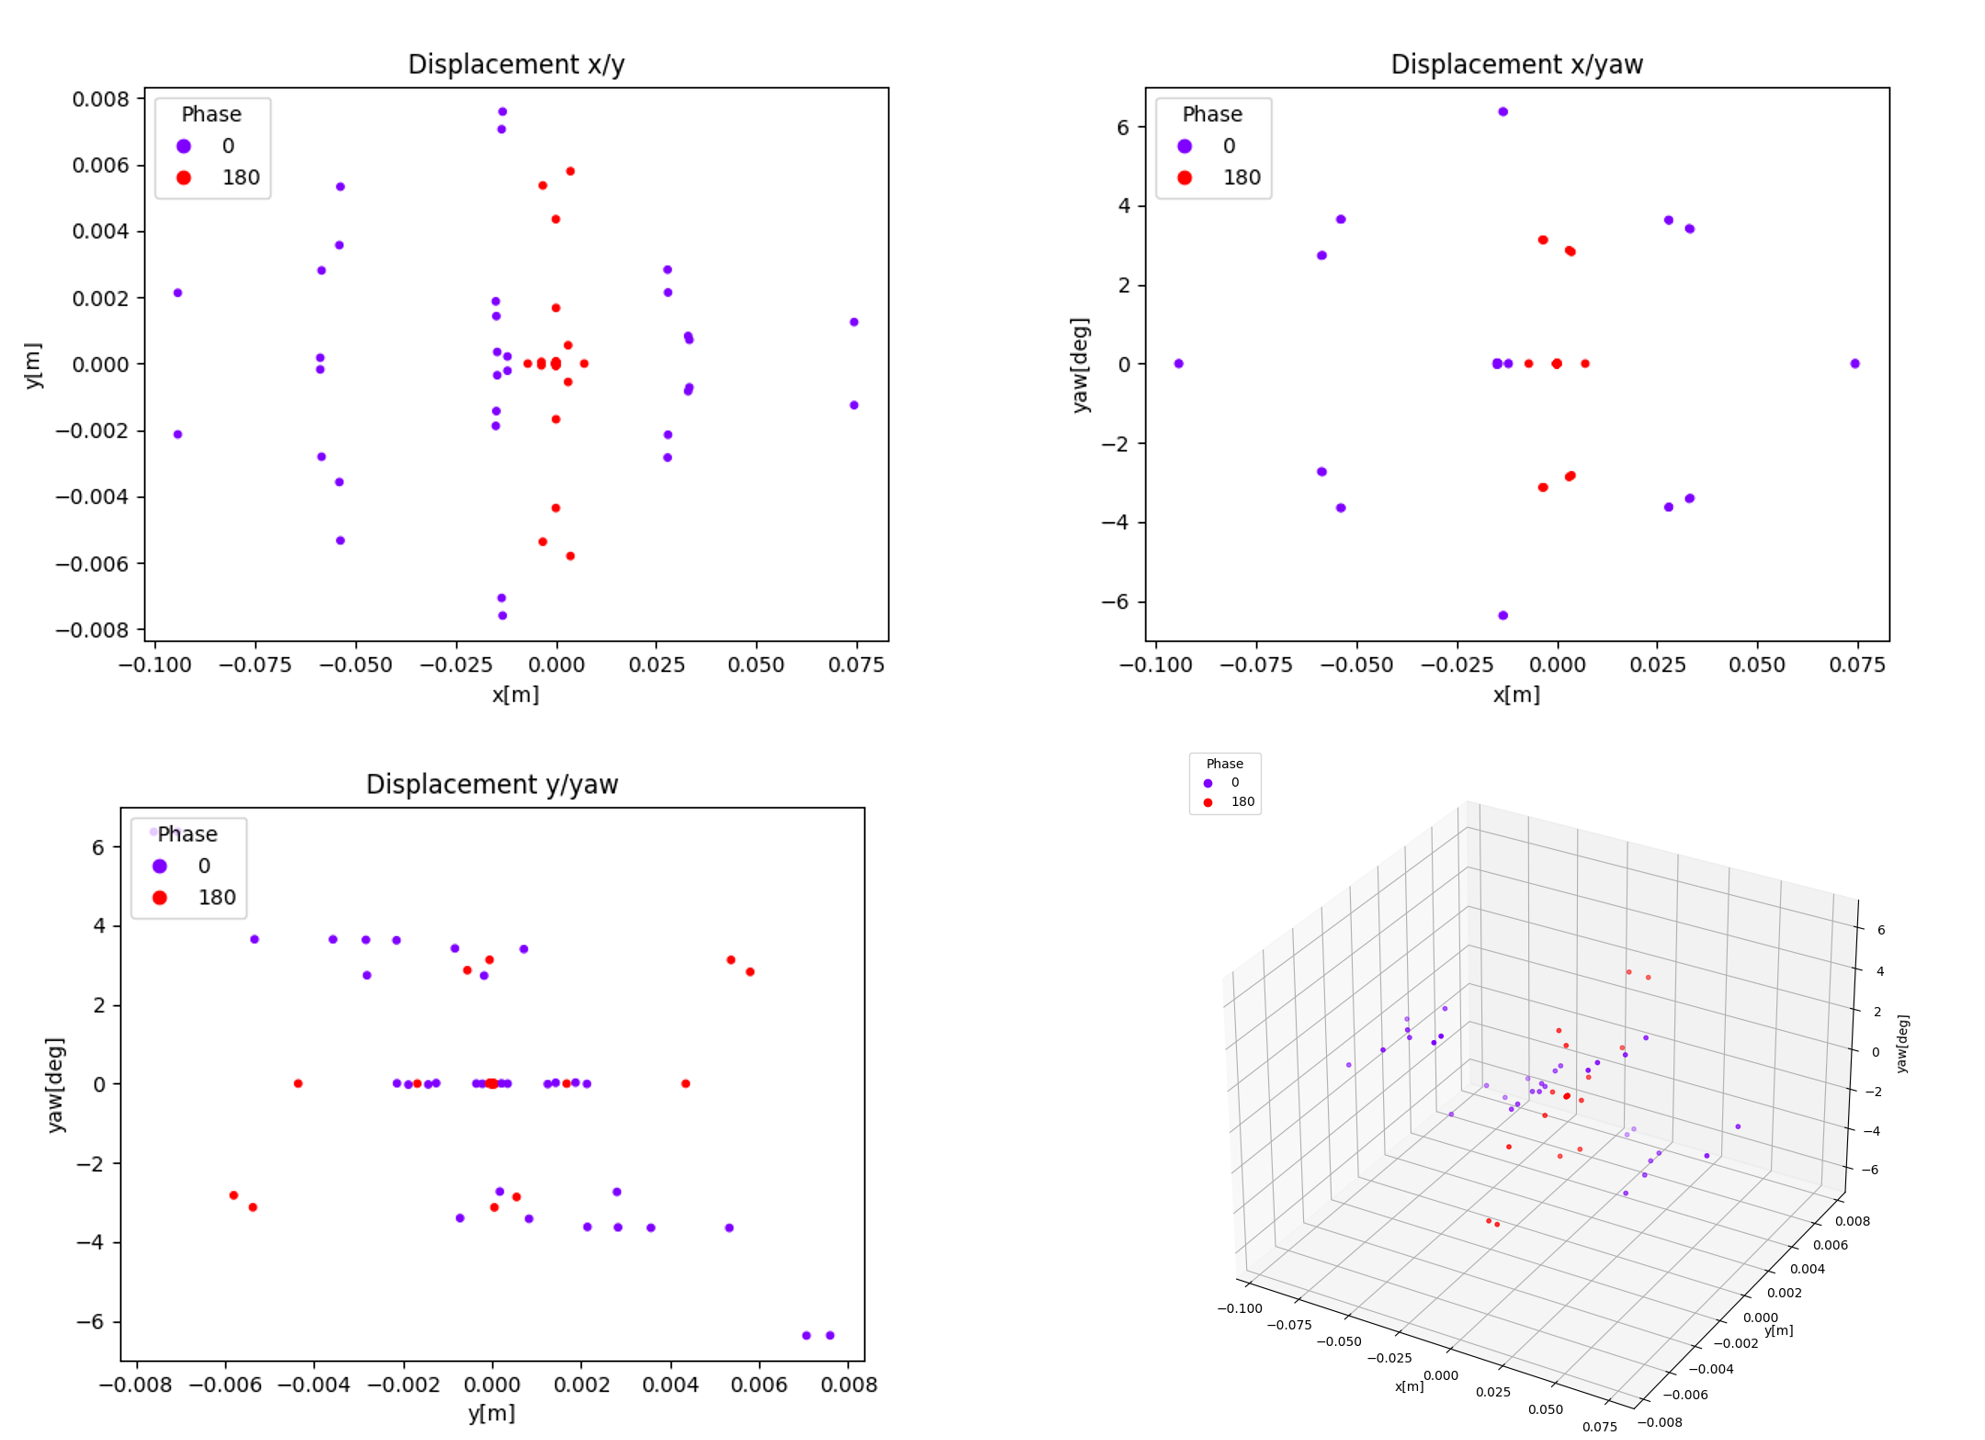
\includegraphics[width=0.7\textwidth]{images/displacement_spread_AB.png}
            \caption{Multiple views of the possible motion of the robot if we restrict it to use only sequences A and B. The robot can move along x-axis and y-axis, but also change its orientation. Bottom right plot shows the 3D view of the position reached for each sequence and phase. Other plots are a projection of those point on only 2 axis. Red dots are sequences with a 180° phase difference while purple dots are sequences with no phase difference.}
            \label{fig:spreadAB}
        \end{figure}
        
        It is also interesting to see that the spread of the points are similar if we limits the possible sequences between sequences A and B as shown on Figure \ref{fig:spreadAB}. As those sequences are experimentally feasible, it would be possible to create a controller that drives the robot only using those specific sequences. The minimum requirement to create a controller for the robot would be to have a forward motion, a backward motion and a turn motion. This seems feasible given the number of different possibilities offered by the sequences and phase differences.\\
        
        The mapping performance is good enough as it is based on the simulation program performances but without the drawing. It takes between 60 minutes and 90 minutes to generate the complete mapping of all the sequences. To generate a subset of sequences, for example sequences A and B, it takes less than ten seconds to generate the table.
        
    \section{Reinforcement Learning Controller}
        As seen on Figure \ref{fig:dqn_results} the robot is able to learn to drive itself using a Deep Q Learning controller. On the Figure \ref{fig:dqn_results} there is a strong progression during the first ten iterations where the number of steps decrease up to around 225 steps per iteration. Between ten and twenty iterations, there is a strong improvement in the number of sequences that switch during an iteration. This number decrease from around 300 to around 50 switches per iteration. In this phase, we can deduce that the neural network is maximizing its reward by reducing the number of switch while keeping the orientation and distance reward constant. After around 40 iterations, both lines reach their limits and stabilize around 200 steps per iterations for around 35 switches per iterations.\\
        
        The associated videos shows that the controller is using most of the potential it has and stop performing unnecessary displacement. It is also interesting to observe that it does work with a subset of selected sequences such as sequences A and B, but the neural net is also able to create an efficient controller with more sequences. This imply to add a hidden layer and change the shape of it to have a first hidden layer with 64 nodes and a second hidden layer with 32 nodes for example. Figure \ref{fig:all_sequences} is an example of Deep Q Learning controller that has access to all the possible sequences. The learning rate is as expected slower than with less sequences as the number of states is larger. Also with a simple neural network as implemented the converging performance is not as good as when restricting to sequences A and B. This can be improved using a larger neural network.\\
        
        The performance of the controller is good enough as the plateau point is reached after around 40 iterations, which happens in less than five minutes of live simulation. The time will be longer if all the sequences are passed as possible action instead of the limitation with sequences A and B and the use of a GPU would be prefered.
        